\documentclass{article}
\usepackage{amsmath,graphicx,float}
\renewcommand\thesection{}
\renewcommand\thesubsection{}

\begin{document}

\title{Intro to Cosmology Homework Solution - Week 1}
\date{}
\maketitle
\section{Ryden 2.2}
The average distance of an unobstructed line of sight through the sky is analagous to the average distance a particle would travel before colliding with another particle. Therefore, we can use the equation for mean free path $l=\frac{1}{n\sigma}$, where $n$ is the 
number density of particles and $\sigma$ is the cross-sectional area of the particles. Using $n=n_{\star}$ and $\sigma=\pi R_{\star}^2$, we have:

\begin{equation*}
l = \frac{1}{10^9 {\rm Mpc}^{-3}\pi (7\cdot10^8{\rm m}\cdot\frac{1~{\rm Mpc}}{3.09\cdot10^{22}{\rm m}})^2} = 6.19\cdot10^{17}{\rm Mpc}
\end{equation*}

for galaxies:

\begin{equation*}
l = \frac{1}{1 {\rm Mpc}^{-3}\pi (2\cdot10^3{\rm pc}\cdot\frac{1~{\rm Mpc}}{10^{6}{\rm pc}})^2} = 7.96\cdot10^{4}{\rm Mpc}
\end{equation*}

\section{Ryden 2.3}

For an object in space, the number of CMB photons to pass through its surface will depend on the density of photons, surface area of the object, and the speed at which they are traveling. We'll let our object be a spherical human of radius 1m for simplicity. If we consider the number of photons existing in a shell of width $\Delta x$ around the surface of the sphere, the number of photons in the shell at that instant will be:

\begin{equation*}
{\rm N_{photons}} = 4.11\cdot10^8 \rm{\frac{photons}{m^3}}\times 4\pi ({\rm 1m})^2 \times \Delta x
\end{equation*}

The number of photons passing through width $\Delta x $ in time $\Delta t$ is simply: 
\begin{equation*}
\frac{{\rm N_{photons}}}{\Delta t} = 4.11\cdot10^8 \rm{\frac{photons}{m^3}}\times 4\pi ({\rm 1m})^2 \times \frac{\Delta x}{\Delta t}
\end{equation*}

Since $\frac{\Delta x}{\Delta t} = c$ for a photon:

\begin{equation*}
\frac{{\rm N_{photons}}}{\Delta t} = 4.11\cdot10^8 \rm{\frac{photons}{m^3}}\times 4\pi ({\rm 1m})^2 \times 3\cdot10^8{\rm \frac{m}{s}} = 1.55\cdot10^{18}~\frac{photons}{s}
\end{equation*}

To calculate how much power is being absorbed by this number of photons, we multiply the above by the average energy per photon:

\begin{equation*}
P = 1.55\cdot10^{18}{\rm \frac{photons}{s}}\times6.34\cdot10^{-4}{\rm\frac{eV}{photon}}\times{\rm \frac{1.6\cdot10^{-19}J}{eV}} = 1.57\cdot10^{-4}\rm W
\end{equation*}

An object that changes its temperature by $\Delta T$ changes its amount of energy by $ \Delta E = Cm\Delta T$. For a time interval $\Delta t$, this is equivalent to $P\Delta t = Cm\Delta T$. Using an average human mass of $\rm m=60kg$, the amount of time it will take to increase their temperature can be calculated by:

\begin{equation*}
\Delta t = \rm \frac{Cm\Delta T}{P} = \frac{4200\frac{J}{kg~K}\times60kg \times 10^{-9} K}{1.57\cdot10^{-4}Js^{-1}} = 1.6s
\end{equation*}



\section{Problem 3}

\subsection{a}
Using the Hubble Law $d = v/H_{0}$:
\begin{equation*}
\rm d =  \frac{14,000~km~s^{-1}}{70~km~s^{-1}Mpc^{-1}} = 200~Mpc
\end{equation*}

\subsection{b}
Using the Hubble relationship $d = cz/H_{0}:$
\begin{equation*}
\rm z = H_{0}d/c = \frac{70~km~s^{-1}Mpc^{-1}\times200~Mpc}{3\cdot10^5~km~s^{-1}} = .047
\end{equation*}
\newpage
\subsection{c}
Using the distance and velocity values from the Hubble Paper, I created the following plot:
\begin{figure}[H]
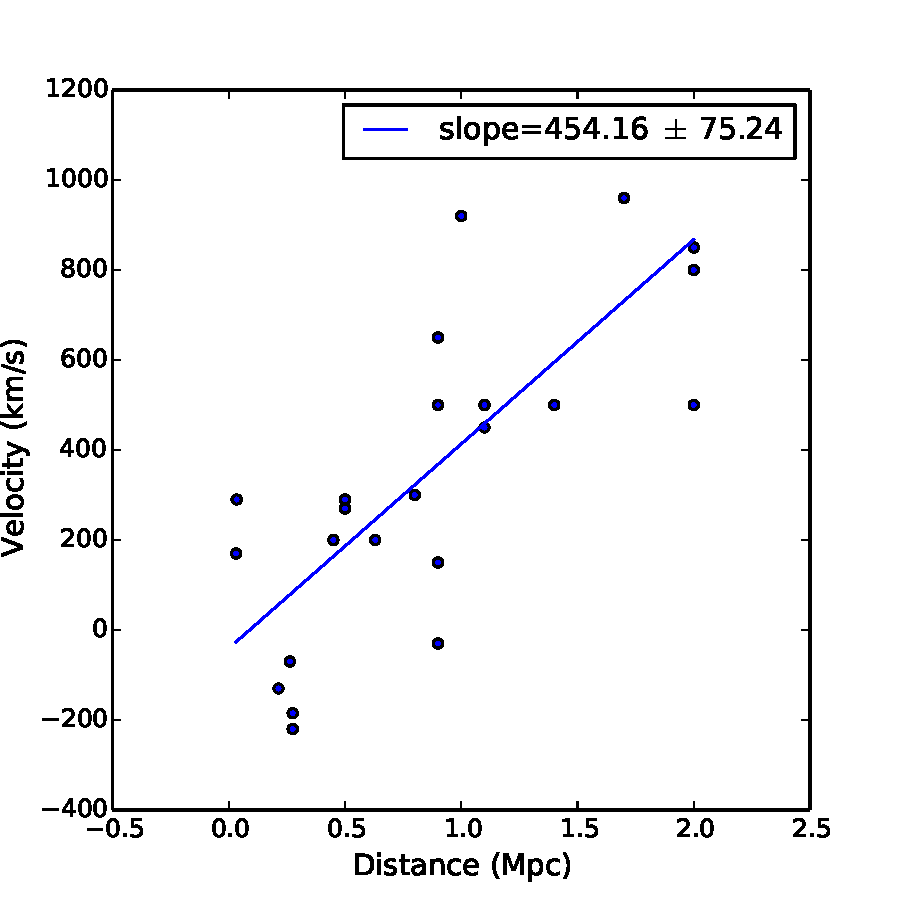
\includegraphics[width=4in]{HW1_plot}
\end{figure}

This gave me a value of $H_{0} = 454~km~s^{-1}~Mpc^{-1}$, which is an order of magnitude greater than what today's measurements suggest.





\subsection{d}
To obtain modern values of distances to galaxies, I used the NASA/IPAC Extragalactic Database (NED)  http://ned.ipac.caltech.edu/forms/byname.html. By typing in the name of a galaxy from Hubble's table (ex NGC 6822), I could then select the "Redshift-Independent Distances" link to get a list of measurments to distance that were not derived from Hubble's Law. Doing this for 10 galaxies, I recreated the plot: 
\begin{figure}[H]
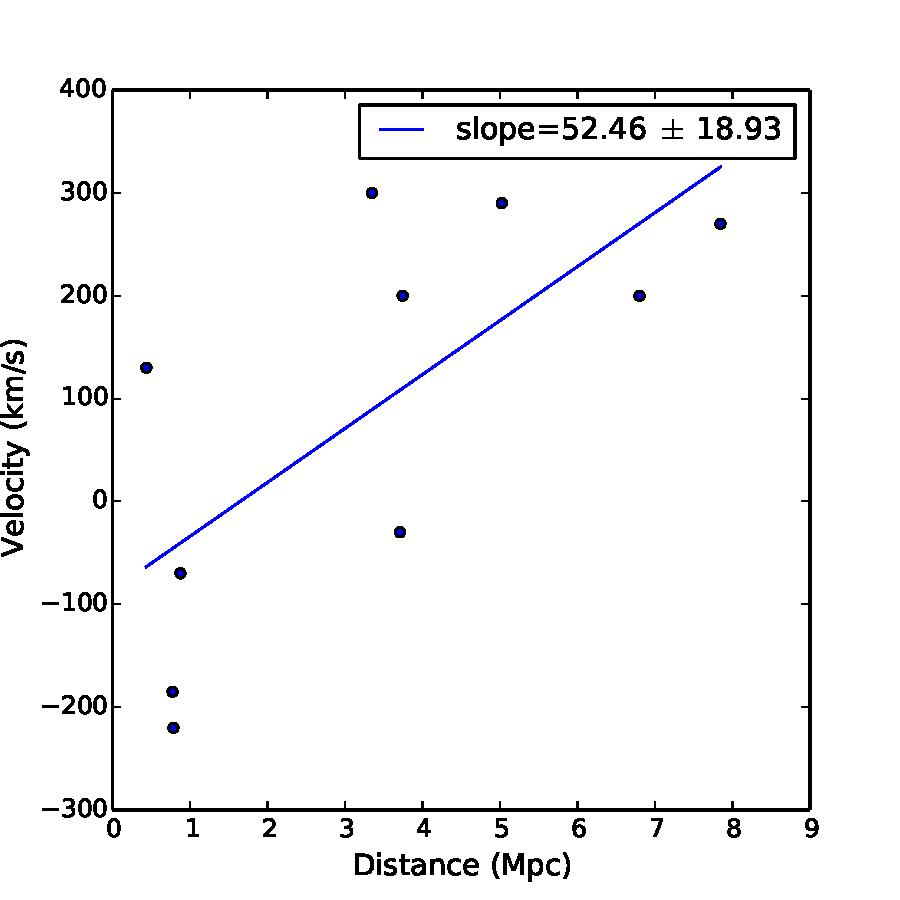
\includegraphics[width=4in]{HW1_plot2}
\end{figure}


This gave me a value of $H_{0} = 52~km~s^{-1}~Mpc^{-1}$, which is much closer to the current result of 67 $km~s^{-1}~Mpc^{-1}$.

\end{document}
